\documentclass[a4paper,11pt]{report}

\author{Florian~Hirtz}
\title{DUMMY: Entwicklung einer Applikation für Mobiltelefone zur Vermittlung von Nachhilfe}

\usepackage[ngerman]{babel}
\usepackage[utf8]{inputenc}
%Linux
%\usepackage[latin1]{inputenc}
\usepackage{blindtext}
\usepackage{graphicx}

%minimale page header & footer
\usepackage{fancyhdr}
\pagestyle{fancy}
\setlength{\headheight}{14pt} 
\fancyhf{}
\fancyhead[C]{\nouppercase{\leftmark}}
\fancyfoot[C]{\thepage}

%Depth of sections
\setcounter{secnumdepth}{3}
\setcounter{tocdepth}{3}
\bibliographystyle{abbrv}

%links
\usepackage{hyperref}

\begin{document}
	\maketitle
	\tableofcontents
	
	
	%VORWORT
	\chapter{Vorwort}
	DummyText...
		\section{Motivation}
		DummyText...
		\section{Danksagungen}
		DummyText...
	
	%Einleitung
	\chapter{Einleitung}
		\section{Zielsetzung}
		Das Ziel dieser Arbeit ist das Entwickeln einer Applikation für Android Geräte, die die Vermittlung von Nachhilfe unter Schülerinnern und Schülern vereinfachen soll. Die Benutzerinnen und Benutzer der Applikation sollen in der Lage sein, sich einen Account innerhalb der Applikation zu erstellen und sich darin einzuloggen. Sie sollen angeben können, in welchen Fächern sie in der Lage sind, anderen Nachhilfe zu geben. Weiter soll eine Funktion vorhanden sein, mit welcher nach anderen Benutzern gesucht werden kann, die in den gewünschten Fächern Nachhilfe anbieten. So sollen Benutzerinnen und Benutzer bei Bedarf gezielt nach Nachhilfelehrern suchen können, die ihren Bedürfnissen entsprechen. Weiter soll es ihnen möglich sein, über eine Chatfunktion andere Benutzer zu kontaktieren.
	
	%Konzeptionelle Grundlagen
	\chapter{Konzeptionelle Grundlagen} \label{konzepte}
		\section{Client-Server Prinzip}
		Das \emph{Client-Server Prinzip} ist ein weit verbreitetes Konzept, um die Aufgaben innerhalb eines Netzwerkes effizient aufzuteilen. Dabei werden die Aufgaben auf zwei im Netzwerk agierende Programme aufgeteilt. Diese Programme werden im Allgemeinen als Client und Server bezeichnet.
	 
		Der \emph{Server} hat die Aufgabe, verschiedenste Dienste zur Verfügung zu stellen, welche auf Anfrage ausgeführt werden können. Ein solcher Dienst kann zum Beispiel das Versenden einer Nachricht oder das Aufrufen einer Webseite sein. Der Server selbst ist passiv. Ein Server sollte immer in der Lage sein, Anfragen entgegenzunehmen und zu verarbeiten.
	
		Der \emph{Client} selber ist die aktive Komponente des Systems. Er ist in der Lage, Anfragen an den Server zu stellen und von dessen Diensten Gebrauch zu machen.
		Grundsätzlich gibt es in einem solchen Netzwerk nur einen Server, jedoch kann es durchaus mehrere Clients geben. Ein guter Server sollte also auch darauf vorbereitet sein, mehrere Anfragen von verschiedenen Clients parallel zu bearbeiten. \cite{fachadmin.de:ServerClient}
		
		%TODO BILD VON SCHEMA SERVER-CLIENT
		
		\section{Das Modell-View-Presenter Konzept (Passive View)} \label{mvp}
		Das \emph{Modell-View-Presenter} (MVP) Konzept wie auch auch das sehr ähnliche \emph{Modell-View-Controller} (MVC) Konzept, sind beide für das Entwickeln von Software entworfen worden. Ihre Idee ist es, die Aufgabenbereiche innerhalb einer Applikation strikt voneinander zu trennen. Dabei wird zwischen drei Typen von Aufgabenbereichen unterschieden:
		\begin{itemize}
			\item Die \emph{View} ist die sichtbare Benutzeroberfläche. Sie hat die Aufgabe, dem Benutzer ein bedienbares Interface zu bieten und soll auf Anfrage den Status seiner einzelnen Komponenten weitergeben . Sie kennt das Model nicht.
			\item Das \emph{Model} ist der Datenspeicher einer Applikation, der gebraucht wird um die View korrekt darzustellen. Es soll auf Anfrage hin Daten ausgeben können. In diesem Falle kennt das Model weder die View noch den Presenter. Je nach Auslegung des Konzepts hat das Model jedoch auch die Aufgabe, falls sich Datensätze ändern, den Presenter davon zu unterrichten. Das Model kennt in diesem Falle zwar das Model, jedoch die View nicht.
			\item Der \emph{Presenter} oder \emph{Controller} ist sozusagen der Mittelmann der beiden anderen Komponenten. Er ist in der Lage Daten aus dem Model anzufordern und kontrolliert anschliessend, was mit diesen Daten geschieht. Er hat ebenfalls die Möglichkeit, die angezeigte View zu ändern und deren Status abzufragen. Der Presenter ist in der Lage, sowohl die View zu manipulieren, als auch das Model.
		\end{itemize}
		Wichtig bei dem MVP Konzept mit einem passiven View ist es, dass nur der Presenter die Möglichkeit hat, auf die beiden anderen Komponenten zuzugreifen. Der View und das Model sollen unter keinen Umständen direkt miteinander kommunizieren. Sämtlicher benötigter Informationsaustausch soll stets vom Presenter kontrolliert werden.\cite{mvp} Ein grosser Vorteil einer nach diesen Regeln entwickelter Applikation ist, dass die einzelnen Komponenten weitgehend unabhängig von einander sind. Somit kann zum Beispiel der View komplett neu gestaltet werden, ohne dass der Presenter oder das Modell geändert werden müssen, damit die Applikation weiterhin funktioniert.
		
		%TODO BILD VON MVP MODELL
		
	\chapter{Die Entwickelte Applikation}
	Die im Rahmen dieser Arbeit entwickelte Applikation wurde für Mobiltelefone mit einer Version des Betriebssystems Android entwickelt. Sie kann darauf installiert und anschliessend ausgeführt werden. Für den Gebrauch der Applikation ist einzig eine Verbindung zum Internet notwendig.
	
	\section{Features}
	Damit die Applikation auch die aufgegebenen Aufgaben erfüllen kann, besitzt sie eine Reihe von Features von welchen Benutzer/Benutzerinnen Gebrauch machen können.
	
	\begin{itemize}
		\item Das \emph{Account-Feature}: Die Applikation bietet den Benutzern/Benutzerinnen die Möglichkeit, sich einen persönlichen Account zu erstellen und ihn zu Personalisieren. Es ist ihnen möglich, auf ihrem Profil ihren Namen, ihre besuchte Schule und ihr Geburtsjahr anzugeben. Weiter können sie auch noch eine kurze Beschreibung von sich selber schreiben und sie haben die Möglichkeit, falls sie selber Nachhilfe anbieten wollen, Fächer auszuwählen, in welchen sie das tun möchten. Das Profil selber ist für andere Benutzer/Benutzerinnen einsehbar. Die meisten Accountdetails können über die Applikation auch noch nach der Registrierung jederzeit bearbeitet werden.
		\item Das \emph{Such-Feature}: Es ist registrierten Benutzern/Benutzerinnen möglich, über eine Suchfunktion nach anderen registrierten Benutzern zu suchen. Dabei kann nach bestimmten Namen gesucht werden oder nach ausgewählten Fächern. Die gefundenen Profile der verschiedenen Benutzern/Benutzerinnen können anschliessend angesehen werden.
		\item Das \emph{Chat-Feature}: Sollte der Benutzer/die Benutzerin einen anderen Benutzer oder Benutzerin gefunden haben, mit welchem/welcher er/sie kontakt aufnehmen möchte, so kann eine Chat via das Gefundene Profil geöffnet werden. Darin können dann in Echtzeit miteinander kurze Textnachrichten ausgetauscht werden. Sollte ein Chat geöffnet sein, können sowohl Sender/Senderin sowie Empfänger/Empfängerin ganz einfach von ihrem eigenen Profil auf ihn zugreifen.
	\end{itemize}
	
	%Projektentwicklung
	\chapter{Applikationskomponenten}
	In diesem Kapitel wird auf die entwickelte Applikation eingegangen. Die einzelnen in der Applikation verwendeten Elemente sollen erklärt werden und ihre Rolle in der entwickelten Applikation ersichtlich werden.
		\section{Systemüberblick}
		Die Applikation wurde nach dem Client-Server Prinzip entworfen und entspricht weitgehend dem MVP Konzept (siehe Kapitel \ref{konzepte}). Der Presenter und die View finden sich beide auf Seiten des Clients (siehe Kapitel \ref{client}) während das Model sich in Form der beiden Server wiederfindet (siehe Kapitel \ref{server} und \ref{fb}).
		
		%Die Server
			\section{Datenbank Server} \label{server}
			Eine der wohl wichtigsten Aufgaben von Computern ist das Speichern, Verwalten und auch Manipulieren von Informationen. Anwendungen, die sich hauptsächlich mit dieser Aufgabe beschäftigen werden allgemein als \emph{Datanbanken} bezeichnet. Sie haben die Aufgabe, Informationen systematisch zu ordnen, zu speichern und bei Bedarf zu verändern. Grundsätzlich bezeichnet der Begriff Datenbank gleich zwei Dinge auf einmal. Zum einen wird ein strukturierter Speicher von Informationen als Datenbank bezeichnet und zum anderen jedoch auch die Anwendung, die das Verwalten der Daten überhaupt erst ermöglicht. Solche Anwendungen werden auch als \emph{Database Management System} (DBMS) bezeichnet und sind meist hochkomplex in ihren Funktionsweisen. \cite{IT-Handbuch}
			
			Datenbanken selbst wiederum können in  verschiedene Typen eingeteilt werden, die alle ihre eigenen Vor- und Nachteile mit sich bringen. Die einfachste Form eines Datenbanktyps ist wohl die \emph{Einzeltabellendatenbank}. Sie besteht aus nur einer Tabelle, in welcher alle Informationen abgespeichert werden. Sie eignet sich gut für kleine, übersichtliche Tabellenstrukturen wie zum Beispiel eine einfache Liste von Adressen. Die Einzeltabellendatenbank stösst jedoch spätestens dann an ihrer Grenzen, wenn die Informationen nicht mehr in nur einer, sondern gleich mehreren Tabellen gespeichert werden. Hier tritt ein anderer Datenbanktyp ins Spiel. Eine \emph{relationale Datenbank} ist in der Lage, verschiedene Tabellen logisch miteinander zu verknüpfen und sich darin zu orientieren. Diese logische Verknüpfung ist möglich aufgrund eindeutigen Eigenschaften eines Eintrags. Dies kann zum Beispiel eine Kundennummer oder ein Name sein. Ein solches Feld wird auch als ein \emph{Key} bezeichnet. Wichtig dabei ist, dass jeder Key nur einmal in einer Tabelle vorkommt, da ansonsten keine eindeutige Verknüpfungen möglich sind. Die Anwendung zur Verwaltung einer solchen relationalen Datenbank wird \emph{Relational Database Management System} (RDBMS) genannt. \cite[S. 745 - 751]{IT-Handbuch}

				\subsection{MySQL Datenbank}
				%TODO GLOSSARY WORK ON LICENCE
				%TODO MySQL ODER MariaDB
				Ein Beispiel für ein solches RDBMS ist die weit verbreitete MySQL Datenbank. Das System wurde ursprünglich von den drei Gründern Allan Larsson, Michael Widenius und David Axmark 1995 entwickelt, wurde später von \emph{Sun Microsytems} aufgekauft und gelangte schlussendlich in den Besitz des amerikanischen Softwareherstellers \emph{Oracle}. MySQL ist unter einem dualen Lizenzsystem eingetragen, sodass die Software zum einen unter einer \emph{General Public Licence} (GPL), aber auch unter eine proprietäre Lizenz gestellt ist. \cite{tecmint.com} Das MySQL System darf aufgrund der GPL gratis heruntergeladen, installiert und modifiziert werden.
				
				In Kombination mit der Programmiersprache PHP bildet sie eines der meist verwendeten Datenspeichersysteme für Webdienste aller Art. Im Falle eines solchen Webdienstes befindet sich die Datenbank meist auf einem zentralen Server, auf welchem sich ebenfalls die benötigten PHP-Skripte befinden. Die PHP-Skripte haben die Aufgabe, Abfragen von den Clients entgegenzunehmen und über sogenannte \emph{Queries} (Datenbank Abfragen) auf die Informationen in der Datenbank zuzugreifen. Im Falle einer MySQL Datenbank werden solche Queries in der Datenbanksprache \emph{SQL} formuliert. Queries können in vier Arten von Abfragen unterteilt werden: \cite[S. 760]{IT-Handbuch}
				
				\begin{itemize}
					\item Auswahlabfragen (\emph{Select Queries}) geben den Inhalt von einem oder mehreren Feldern aus einer oder verschiedenen Tabellen zurück. Dabei kann bei Bedarf nach Kriterien gefiltert werden, um die Suche nach bestimmten Datensätzen einzugrenzen.\cite[S. 746]{IT-Handbuch}
					\item Einfügeabfragen (\emph{Insert Queries}) fügen einen neuen Datensatz zu einer bestehenden Tabelle hinzu.\cite[S. 746]{IT-Handbuch}
					\item Änderungsabfragen (\emph{Update Queries}) ändern bestimmte oder alle Felder eines bestehenden Datensatzes in einer Tabelle.\cite[S. 746]{IT-Handbuch}
					\item Löschabfragen (\emph{Delete Queries}) löschen einen Datensatz aus einer Tabelle. \cite[S. 746]{IT-Handbuch}
				\end{itemize}
				
				\subsection{MySQL Datenbankstruktur} \label{databankstructure}
				
				\begin{figure}
					\begin{center}
						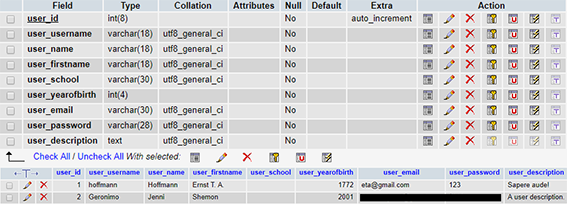
\includegraphics{user_archive.png}
						\caption{Die user\_archive Tabelle, aufgenommen aus dem phpMyAdmin Interface}
						\label{user_archive:PNG}
					\end{center}
				\end{figure}
				\begin{figure}
					\begin{center}
						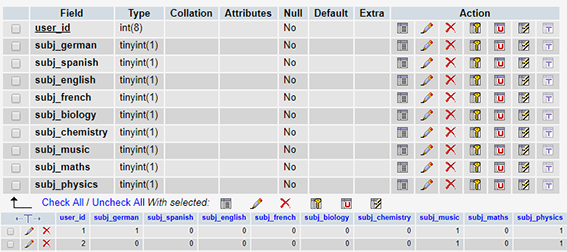
\includegraphics{user_subjects.png}
						\caption{Die user\_subjects Tabelle, aufgenommen aus dem phpMyAdmin Interface}
						\label{user_subjects:PNG}
					\end{center}
				\end{figure}
				\begin{figure}
					\begin{center}
						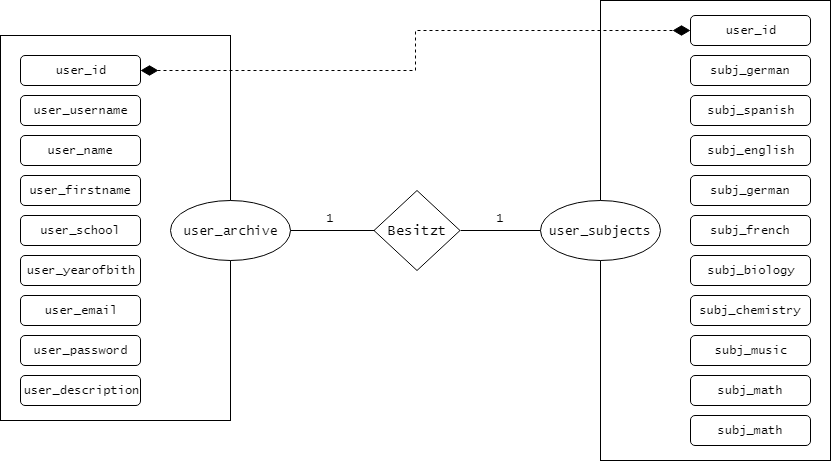
\includegraphics[width=0.8\textwidth]{ERM-Matura.png}
						\caption{Das ERM der entwickelten Applikation.}
						\label{ERM}
					\end{center}
				\end{figure}
				
				%TODO REWRITE AND STRUCTURE
				%In der entwickelten Applikation wird genau ein solches MySQL Datanbanksystem in Kombination mit PHP (siehe Kapitel \ref{ssec:PHP}) benutzt. Die Datenbank wird verwendet, um die Accountdaten der einzelnen Benutzer zu speichern und den Clients zur Verfügung zu stellen. Sie befindet sich auf dem Schulserver vom Ergänzungsfach. Die Datenbank selber umfasst zwei miteinander verknüpfte Tabellen. Die eine läuft unter dem Name \emph{user\_archive} (siehe Abbildung \ref{user_archive:PNG}) und beinhaltet die essentiellen Accountdetails wie Name, Email, Passwort etc. Zu erwähnen ist hier das erste Feld \emph{user\_id}. Es wird bei einem neuen Eintrag in die Tabelle automatisch generiert (\emph{auto\_increment}) und gewährt so, dass sämtliche Einträge eindeutig unterschieden werden können. Ähnlich verhält sich das Feld user\_username. Es ist als \emph{unique} markiert und soll ebenfalls verhindern, dass es beim Login zu Mehrdeutigkeiten kommt. Sie sind die Keys der Tabelle. Die zweite Tabelle der trägt den Namen \emph{user\_subjects} (siehe Abbildung \ref{user_subjects:PNG}). Sie umfasst nebst einem Feld für die user\_id sämtliche momentan von der Applikation unterstützten Fächer. In den Feldern wird nun mithilfe von 1 und 0 angegeben, welche Fächer von einem Benutzer/ einer Benutzerin angewählt wurden, also in welchen er/sie andere unterstützen könnte. Die Inhalte wurden bewusst von einander getrennt, um die Übersichtlichkeit in der user\_archive Tabelle zu wahren. Das user\_id Feld ist auch hier ein Key und ist für jeden Benutzer gleich wie in der user\_archive Tabelle. Diese Verknüpfung der Tabellen kann sehr übersichtlich durch ein \emph{Entity-Relationship-Modell} (ERM) dargestellt werden, da das Modell lediglich zwei Tabellen (Im falle des ERM \emph{Entities}) umfasst. ERMs eignen sich besonders für die Darstellung von Datenbankstrukturen und deren Verknüpfungen. Sie sind oft der erste Schritt, wenn es um die Planung einer neuen Datenbank geht. Die Beziehungen werden durch hauptsächlich zwei Variablen beschrieben, welche im Schema (x, y) dargestellt werden. Die Variable x gibt das Minimum an herrschenden Beziehungen mit anderen Entities vor. Die Variable y das Maximum. Die Variablen können entweder eine bestimmte Zahl wie 1 oder 0 sein oder sie können durch m/n verkörpert werden, stellvertretend für beliebig viele Beziehungen. Im falle des ERMs der entwickelten Applikation (siehe Abbildung \ref{ERM}) ist das eine (1,1) : (1,1) Beziehung. Das bedeutet, dass es in beiden Tabellen jeweils genau einen Eintrag für einen Benutzer gibt. \cite[S. 750]{IT-Handbuch}\cite{ERM}\cite{ERM2}

				In der entwickelten Applikation wird genau ein solches MySQL Datanbanksystem in Kombination mit PHP (siehe Kapitel \ref{ssec:PHP}) benutzt. Die Datenbank wird verwendet, um die Accountdaten der einzelnen Benutzer zu speichern und den Clients zur Verfügung zu stellen. Sie befindet sich auf dem Schulserver vom Ergänzungsfach. Die Datenbank umfasst 2 Tabellen: die \emph{user\_archive} Tabelle und die \emph{user\_subjects} Tabelle. In der user\_archive Tabelle findet sich ein Eintrag für jeden registrierten Benutzer mit Informationen wie Benutzername, Passwort und Jahrgang (siehe Abbildung \ref{user_archive:PNG}). Die andere Tabelle beinhaltet Felder für alle von der entwickelten Applikation unterstützten Fächer (siehe Abbildung \ref{user_subjects:PNG}). Mithilfe der Werte 1 und 0 wird angegeben, in welchen Fächern ein Benutzer/eine Benutzerin Unterstützung anbietet. Die Struktur der Datenbank kann durch ein \emph{Entitiy-Relationship-Modell} (ERM) dargestellt werden. ERMs sollen visualisieren, in welcher Beziehung verschiedene Bestandteile von Datenstrukturen (\emph{Enities}) zu einander stehen. ERMs sind oftmals der erste Schritt wenn es um die Planung einer neuen Datenbank geht. Das ERM der im Rahmen dieser Arbeit benutzen Datenbank ist in Abbildung \ref{ERM} visualisiert. Die Verhältnisse werden im Schema (1, 1) geschrieben. Die erste Ziffer gibt die minimale Anzahl an herrschenden Beziehungen an, die zweite Ziffer die maximale Anzahl. Im Falle von (1, 1) Beziehungen bedeutet dies, dass es immer genau eine solche Beziehung geben darf und auch muss. Sind die Anzahl Beziehungen unlimitiert, steten anstelle der Ziffern stellvertretend die Variablen \emph{m} oder \emph{n}. Die Tabellen sind über den Key user\_id miteinander Verknüpfbar.\cite[S. 750]{IT-Handbuch} \cite{ERM} \cite{ERM2}
				
				Abbildungen von den beiden Tabellen findet sich in den Abbildungen \ref{user_archive:PNG} und \ref{user_subjects:PNG}. Im oberen Teil der Abbildungen sieht man die Konfiguration der einzelnen Felder. In der Spalte \emph{Field} ist der Name der Felder eingetragen. In der Spalte \emph{Type} wird der zugelassene Datentyp des Feldes definiert. Ist der Datentyp eine Form von Text, wird in der Spalte \emph{Collation} die Kodierung der Unicode-Zeichen angegeben. In der Spalte \emph{Extras} können noch eine Reihe von speziellen Eigenschaften den Feldern zugewiesen werden. Eine davon ist die im Feld \emph{user\_id} verwendete \emph{auto\_increment} Funktion. Sie führt dazu, dass neue Einträge in der Tabelle in diesem Feld automatisch durchnummeriert werden. Das Feld user\_id ist in beiden Tabellen als Key markiert. Das heisst, dass das die user\_id von der Datenbank zur eindeutigen Verknüpfung der beiden Tabellen benutzt werden soll. Ebenfalls zu erwähnen ist das Feld \emph{user\_username}. Es ist als \emph{unique} markiert, was heisst, dass es in der Tabelle keine identische Benutzernamen geben darf (siehe Kapitel \ref{login:php}). Im unteren Teil der Abbildung findet sich ein beispielhafter Ausschnitt, wie eine solche Tabelle Aussehen könnte.
				%TODO GLOSSAR OBJEKTORIENTIERT
				\subsection{PHP Skripte} \label{ssec:PHP}
				Nebst dem Datenbanksystem selbst befinden sich ebenfalls diverse PHP Skripte auf dem Server. Sie sind in der Open-Source Skriptsprache PHP geschrieben. PHP ist ein rekursives Akronym für \emph{Hypertext Preprocessor} und ist eine speziell für die Webprogrammierung entwickelte Programmiersprache, welche zu den objektorientierten Programmiersprachen gehört. PHP wird hauptsächlich für die Programmierung innerhalb von Webservern verwendet und bietet den grossen Vorteil, dass Clientbenutzer zwar durchaus die Skripte auf dem Server ausführen, jedoch nicht ansehen können. Sie erhalten lediglich eine Antwort ohne je die Codestruktur des PHP Skriptes zu Gesicht bekommen zu haben.\cite{PHP} Dies ist möglich, da der PHP-Code ausschliesslich serverseitig ausgeführt wird. Ein \emph{Interpreter} führt ihn auf dem Server aus und erst die vom Interpreter generierte Ausgabe wird dem Client als Antwort zugeschickt. Die Antwort ist meist in der Auszeichnungssprache HTML (\emph{Hypertext Markup Language}) verfasst, können jedoch durchaus auch in PDF, JavaScript, JSON oder sogar Bildformaten sein.\cite{PHP:function} Die Website \emph{json.org} (\cite{JSON}) beschreibt JSON wie folgt:
				
				%TODO GLOSSAR PARSEN
				\begin{quotation}
					"JSON (JavaScript Object Notation) ist ein schlankes Datenaustauschformat, das für Menschen einfach zu lesen und zu schreiben und für Maschinen einfach zu parsen (Analysieren von Datenstrukturen) und zu generieren ist.[...]Bei JSON handelt es sich um ein Textformat, das komplett unabhängig von Programmiersprachen ist[...]. Diese Eigenschaften machen JSON zum idealen Format für Datenaustausch."\cite{JSON}
				\end{quotation}
			
				Die im Rahmen dieser Arbeit entwickelte Applikation benutzt für ihre Kommunikation von MySQL Datenbank zu Client ausschliesslich JSON-Formate. Dieses Format eignet sich perfekt für den Austausch von Daten wie sie in der Datenbank gespeichert sind.
				
				%TODO: MB POST ERWÄHNEN BEI ENTGEGENGENOMMENEN BENTZERNAME UND PASSWORT
					\subsubsection{Login}\label{login:php}
					Damit ein Client Zugriff auf einen Datensatz in der Datenbank bekommt, muss sich der Benutzer/ die Benutzerin zuerst unter einem bestehenden Account einloggen. Dabei wird auf dem Client Benutzername (Username) und Passwort eingegeben (siehe Kapitel \ref{login:act}). Daraufhin ruft der Client das Skript \emph{login.php} via Webadresse auf und übergibt ihm Benutzername und Passwort. Das aufgerufene Loginskript erstellt eine Verbindung zur lokalen MySQL Datenbank. Als nächstes wird versucht einen Eintrag in der user\_archive Tabelle zu finden, bei welchem die Felder user\_username und user\_password mit den empfangenen Werten übereinstimmen. Dies wird über ein sogenanntes \emph{MySQL Statement} getan. In diesem Statement wird in der Datenbank nachgefragt, ob es einen Eintrag mit den bestimmten Angaben gibt (Select Query).
					\begin{quotation}
						{\fontfamily{qcr}\selectfont\noindent 'SELECT * FROM user\_archive WHERE user\_username=? AND user\_password=?'}
					\end{quotation}
				
					%TODO REWRITE AND SIMPLIFY
					%Wenn die Suche erfolgreich ist, wird auf das Statement mit dem Inhalt eines Datensatzes geantwortet, welcher dann vom PHP Skript wiederum lokalen Variablen zugewiesen wird. Nun ist auch die user\_id des Benutzers bekannt und es kann über ein zweites Statement den entsprechenden Datensatz aus der user\_subjects Tabelle ausgelesen werden. Wieder werden zurückgegebenen Werte in lokalen Variablen gespeichert. Die Werte aller gespeicherten Variablen werden nun in ein Array mit dem Namen \emph{response} übertragen und ihnen wird jeweils einen \emph{Key} (Zeichen, unter welchem der Wert im Array gespeichert ist) zugewiesen. Ebenfalls wird eine zusätzliche Variable unter dem Key \url{success} mit dem Wert \url{true} in den Array gespeichert. Die Variable \url{success} Teilt dem Client mit, dass die Anfrage erfolgreich war. Ist jedoch die Suche nach einem registrierten Benutzer mit eingegebenen Daten in der Datenbank erfolglos, verfasst das PHP Skript ein JSON Datei mit der Variable \url{response["success"] = false} und fügt keine weiteren Daten mehr an. Schlussendlich wird der Antwortarray mit den gespeicherten Daten in einem JSON Format gespeichert und das erstellte JSON File wird an den Client zurückgeschickt. Damit es beim Login zu keinen Mehrdeutigkeiten kommt ist es von Wichtigkeit, dass jeder Benutzername nur einmal in der Tabelle vorkommt (siehe Kapitel \ref{databankstructure}).
					
					Wenn du Suche erfolgreich ist, wird dem Statement mit dem Inhalt eines Datensatzes geantwortet. Es ist wichtig, dass jeweils nur maximal ein Eintrag dabei gefunden werden kann. Deshalb muss der Benutzername aller Benutzer/Benutzerinnen einzigartig sein (siehe Kapitel \ref{databankstructure}). Mit diesen Informationen kann nun über die user\_id ebenfalls der Datensatz des Benutzers/der Benutzerin aus der Tabelle user\_subject ausgelesen werden. Alle nun erhaltenen Daten aus der Datenbank werden anschliessen im JSON-Format an den Client geantwortet und teilt gleichzeitig auch noch dem Client mit, dass das Login erfolgreich war. Hat die Suche jedoch keine Ergebnisse geliefert, wird dem Client über ein JSON-Format geantwortet, dass das Login fehlgeschlagen ist.
					\subsubsection{Registrierung}
					Wenn ein Benutzer/eine Benutzerin noch keinen Account hat, soll er/sie die Möglichkeit haben, einen zu erstellen. Hierzu kann er/sie auf dem Client die benötigten Daten eingeben (siehe Kapitel \ref{register:act}) und es wird eine Anfrage an das Skript \emph{register.php} auf dem Server geschickt. Dieses Skript hat die Aufgabe in beiden Tabellen einen neuen Eintrag für den Benutzer/die Benutzerin zu erstellen, sofern die Daten legitim sind. Zuerst wird dafür eine Verbindung mit der lokalen Datenbank aufgenommen. War dies erfolgreich, wird ein Auswahlabfrage formuliert, welche nach einem Datensatz mit dem eingegebenen Benutzernamen sucht. Nur wenn kein solcher Datensatz gefunden werden kann, wird fortgefahren, ansonsten wird frühzeitig eine Antwort an den Client geschickt, die ihm mitteilt, dass die Registrierung erfolglos war, da bereits ein Eintrag mit diesem Benutzernamen existiert (siehe Kapitel \ref{login:php}). Wenn kein bestehender Datensatz mit dem gewählten Benutzernamen gefunden worden ist, wird ein SQL Statement vorbereitet, welches einen neuen Datensatz in die Tabelle user\_archive einfügt (Insert Query), und bei welchem sogleich alle vom Benutzer/von der Benutzerin angegebenen Daten in die Felder eingefügt werden. Die Fragezeichen stehen stellvertretend für die einzufügenden Werten, die erst später zugewiesen werden. Mehr dazu in Kapitel (\ref{security}).
					\begin{quotation}
						{\fontfamily{qcr}\selectfont\noindent 'INSERT INTO user\_archive(user\_username, user\_name, [...]) VALUES (?, ?, [...])'}
					\end{quotation}
					
					Als nächstes soll noch ein Eintrag in der user\_subjects Tabelle erstellt werden, welcher die gleiche user\_id hat, wie der soeben neu erfasste Datensatz in der user\_archive Tabelle. Hierzu wird zuerst über ein Statement die von der Datenbank automatisch zugewiesene user\_id aus der user\_archive Tabelle ausgelesen. Daraufhin wird eine weitere Insert Query mit der ausgelesenen user\_id und dem Wert 0 für alle Fächer in die user\_subjects Tabelle gestellt. Der Wert 0 steht in den Feldern stellvertretend für den Wert \url{false}, da neu erstellte Accounts standardmässig keine Fächer ausgewählt haben sollen. Schlussendlich, wird eine JSON Antwort verfasst, welche dem Client eine erfolgreiche Registrierung mitteilt.
					
					
					\subsubsection{Änderungen via Einstellungen vom Client}
					Es soll den Benutzern/Benutzerinnen möglich sein, gewisse Angaben wie Email, Passwort oder die ausgewählten Fächer nachträglich zu verändern. Der Client bietet dafür eine Settings Activity (siehe Kapitel \ref{settings:act}) mit welcher die Angaben editiert werden können. Wenn die editierten Angaben auf dem Client gespeichert werden, wird eine Anfragen an das Skript \emph{savesettings\_pw.php} geschickt. Dieses Skript ist in der Lage bereits bestehende Datensätze in der Datenbank zu verändern und die veränderten Daten zurückzuschicken. Hierzu wird zuerst eine Verbindung mit der Datenbank aufgenommen. Daraufhin wird überprüft, ob die Anfrage auch die Berechtigung für eine solche Änderungsabfrage (Update Query) hat. Im Falle der entwickelten Applikation ist das sehr simpel gelöst. Es wird ähnlich wie beim login.php Skript eine Auswahlabfrage formuliert, die nach einem Datensatz mit einer bestimmten user\_id und Passwort fragt. Das Passwort muss vom Nutzer nicht manuell eingegeben werden, sondern wird im Hintergrund von der Client Applikation automatisch geregelt. Diese Vorkehrung ist aus Sicherheitsgründen sehr wichtig. Sollte das Passwort nicht überprüft werden, wäre es möglich, dass unberechtigte Personen die Datensätze von Benutzern/Benutzerinnen editieren könnten. Ist die Auswahlabfrage erfolgreich, wird zunächst eine Update Query formuliert, welches den Datensatz in der Tabelle user\_archive durch den neuen mit den Aktualisierten Daten ersetzt.
					\begin{quotation}
						{\fontfamily{qcr}\selectfont\noindent 'UPDATE user\_archive SET [...] WHERE user\_id=?'}
					\end{quotation}
					
					Anschliessend wird der Datensatz per Auswahlabfrage wieder Ausgelesen und die Daten in lokalen Variablen gespeichert. Das gleiche mit der user\_subjects Tabelle gemacht. Sämtliche ausgelesenen Daten werden in einen Array gespeichert und dieser wird anschliessend im JSON Format an den Client zurückgeschickt. So wird gewährleistet, dass die lokalen Variablen auf dem Client mit Sicherheit mit denen in der Datenbank übereinstimmen.
					\subsubsection{Suchanfrage} \label{sssec:Suchanfrage}
					Damit es Benutzern/Benutzerinnen möglich ist, nach anderen Benutzern und Benutzerinnen zu suchen, wird ein PHP Skript benötigt, welches die Datenbank nach Datensätzen durchsucht, welche bestimmten Kriterien erfüllen. Diese Kriterien kann der Benutzer/die Benutzerinnen auf dem Client angeben (siehe Kapitel \ref{filter:act}). Es soll nach Namen und nach Fächern gesucht werden können. Das Skript serach.php übernimmt diese Aufgabe. Hierzu wird zuerst eine Verbindung mit der Datenbank aufgebaut. Ist das erfolgreich wird Select Query erstellt, die alle den Kriterien entsprechenden Datensätze zurückliefern soll. 
					
					Das MySQL Statement wird in zwei Schritten erstellt.Im ersten wird ein \emph{String} erstellt der gleich zwei Dinge tut. Zum einen schafft er eine Verknüpfung zwischen den beiden Tabellen user\_archive und user\_subjects. Dies wird durch die SQL Funktion \emph{INNER JOIN} erreicht. Diese Funktion ermöglicht es, die beiden Tabellen über die user\_id (Key) zu verbinden. Nun kann die Select Query in beiden Tabellen gleichzeitig nach mehreren Kriterien suchen und die Ergebnisse direkt zusammenführen.
					\begin{quotation}
						{\fontfamily{qcr}\selectfont\noindent 'SELECT user\_archive.*, user\_subjects.* 
							
						\noindent FROM user\_archive INNER JOIN user\_subjects ON
						
						\noindent user\_archive.user\_id = user\_subjects=user\_id WHERE user\_archive.user\_username LIKE ? OR [...]'}
					\end{quotation} 
					Weiter ist im String auch bereits das Suchkriterium bezüglich des Namens enthalten. Dazu wird die SQL Funktion \emph{LIKE} verwendet. Diese Funktion ermöglicht es, das nach Daten gesucht wird, die den eingegebenen Wert enthalten, jedoch nicht unbedingt komplett identisch sind. Zum Beispiel würde bei der Suche nach einem \glqq Max\grqq{} auch der Datensatz von \glqq Maximilian\grqq{} gefunden werden. Dies ermöglicht es Benutzern/Benutzerinnen auch ein gewünschtes Suchresultat zu finden, wenn sie nicht den exakten Namen kennen. Es kann nach Benutzernamen, Vor- sowie Nachnamen gesucht werden.
					
					Im zweiten Schritt werden an den erstellten String noch die Kriterien für die ausgewählten Fächer angehängt. Dabei werden alle ausgewählten Fächer nacheinander als ein obligatorisches Kriterium an den String angehängt. Das bedeutet, dass wenn nach einer \glqq Magalie\grqq{} gesucht wird und gleichzeitig noch Mathematik als ein Kriterium ausgewählt ist, nur die Datensätze ausgewählt werden, bei welchen zum einen der Name \glqq Magalie\grqq{} vorkommt, aber auch Mathematik als angebotenes Fach markiert ist.
					
					Die Informationen der Suchergebnisse mit Ausnahme des Passwortes werden zuerst einzeln in eigenen Arrays gespeichert. Nun werden alle diese Arrays durchnummeriert in einen weiteren Array gespeichert. So sind alle Suchergebnisse kompakt und systematisch geordnet und können als ein einzelnes Element im Antwortarray referenziert werden. Nun wird noch der Wert \url{true} mit dem Key \url{"success"} im Antwortarray gespeichert und das ganze als JSON Datei dem Client zurückgeschickt.
					
					
			%TODO GLOSSAR API
			\section{Firebase} \label{fb}
			Firebase ist eine  Entwicklungsplattform für Webapplikationen, welche seit 2014 von Google angeboten wird. Firebase entwickelte sich aus dem 2011 gegründete Startup \emph{Envolve} der beiden Gründern James Tamplin und Andrew Lee. Das Ziel von Envolve war es, Kunden eine API (\emph{Application Programming Interface}) zu bieten, mit welcher Realtime Chatfunktionen einfach realisiert werden können. Nachdem jedoch viele Benutzer die API für andere Anwendungen als Chats verwendeten, ja sogar einzelne Spielentwickler sie für eine Realtime Synchronisation verschiedener Clients verwendeten, begann die Entwicklung sich auf das Anbieten einer API für Realtime Service zu konzentrieren. Der Erfolg war gross und 2014 wurde Google darauf aufmerksam und kaufte das Unternehmen auf. Google entwickelte aus Envolve daraufhin eine Plattform, welche verschiedenste Tools zur Webdienstentwicklung beinhaltet und heute unter dem Namen Firebase vermarktet wird. Firebase bietet sowohl Tools für die Entwicklung neuer Dienste wie Realtime Datenbanken, Authentifizierungsfunktionen und Crashanalysen, aber auch für das Unterhalten von bestehenden Servicen. Beispiele für ein solche Tools zur Unterhaltung bestehender Dienste wären zum Beispiel das Senden von Push-Benachrichtigungen an alle Clients oder das Überwachen von geschalteter Werbung innerhalb der Clients. Die Tools dürfen in einem begrenzten Rahmen gratis verwendet werden und sind daher sehr attraktiv für kleinere Entwicklerunternehmen, jedoch durchaus auch für grössere Unternehmen.\cite{Firebase}
				
				\subsection{Firebase Realtime Datenbank} \label{realtime}
				Wie bereits erwähnt, bietet Firebase unter anderem auch Realtime Datenbankfunktionen an. Die Firebase Realtime Datenbank (RTDB) ist eine NoSQL Datenbank und unterscheidet sich in ihrer Funktionsweise stark von relationalen Datenbanken. Anders als relationale Datenbanken agieren Echtzeitdatenbanken nicht nur Passiv auf Anfrage sondern teilen den Clients aktiv mit, wenn sich ein Datensatz verändert hat (Push-Based Data Access) und halten ihn so immer auf dem neusten Stand. Echtzeitdatenbanken werden besonders dann eingesetzt, wenn sich ein Datensatz häufig oder jederzeit ändern kann und es notwendig ist, dass die Clients ohne grosse Verzögerung davon unterrichtet werden.\cite{RealtimeDatabase} Es ist dann nicht einmal nötig, das die Clients zur Zeit des Pushes online sind. Sie werden bei Start automatisch mit dem Datensatz auf der Datenbank abgeglichen und aktualisiert.\cite{FirebaseRTDB}
				
				Die Chatfunktion in der entwickelten Applikation ist ein genau solcher Dienst, der eine solche Datenbank benötigt. So können Clients in Echtzeit miteinander Kommunizieren, ohne dass sie permanent online sein müssen, oder die Applikation konstant Anfragen an den Server nach neu empfangenen Nachrichten schicken muss. Die Wahl für die Firebase Plattform ist dann einfach gewesen. Der Client ist im ebenfalls von Google entwickelten Android Studio entwickelt worden. Android Studio Unterstützt standardmässig die Firebase API, weshalb das Einbinden einer Firebase RTDB in eine Applikation sehr einfach ist (siehe Kapitel \ref{chat:act}).
				
				%TODO BILD VON FIREBASE
				\subsection{Firebasestruktur}
				Firebase Echtzeitdatenbanken haben eine andere Struktur als relationale Datenbanken. Die Informationen sind nicht in Form von Tabellen gespeichert sondern können vielmehr mit der Struktur eines Ordnersystems verglichen werden. Der Ort, wo die Informationen gespeichert sind, wird in Pfaden angegeben, die mit denen eines Filesystems eines Computers vergleichbar sind. Dabei gibt es einen Hauptordner, der sozusagen die gesamte Datenbank umfasst. Diese wiederum hat Unterordner, welche im Allgemeinen als \emph{Children} bezeichnet werden.
				
				Die Struktur der im Rahmen diese Arbeit benützen Datenbank besteht aus zwei Ordnern, dem \emph{User}-Ordner und dem \emph{Chats}-Ordner. Im User Ordner	sind alle Benutzer verzeichnet, die einen oder mehrere offene Chats besitzen. Der Ordner dient dazu, offene Chats eines Benutzers auf der Hauptseite des Clients darzustellen und öffnen zu können. Die Children des Verzeichnis sind unter den user\_ids der Benutzer gespeichert. Für jeden offenen Chat findet sich in einem solchen Child nun ein weiteres Child für jeden offenen Chat des Benutzers/der Benutzerin. Dieses enthält die eigentlichen Informationen, die für das Öffnen und Darstellen des Chats benötigt werden. Ebenfalls enthalten sie auch den Pfad des eigentlichen Chats, wo auch die Nachrichten gespeichert sind (siehe auch Kapitel \ref{warum}). Die offenen Chats findet man alle im Chats Verzeichnis. Dort sind als Children alle Chats zu finden. Der Name wird ihnen durch die beteiligten Chatpartner/Chatpartnerinnen gegeben. Das heisst, ein Chat zwischen der Benutzer A mit der ID 9 und einer Benutzerin B mit der user\_id 21 würde unter dem Namen 9\textgreater\textgreater21 zu finden sein. Im Chatverzeichnis selber befinden sich alle gesendeten Nachrichten. Der Name der Nachrichten wird von Firebase selber generiert. Die Nachrichten enthalten nun die drei eigentlich versendeten Werte: die Nachricht, das Sendedatum und Uhrzeit und den Absender/die Absenderin.
				
				\subsubsection{Warum genau diese Struktur?} \label{warum}
				Es ist an dieser Stelle noch interessant zu erwähnen, weshalb die Firebasestruktur auf den ersten Blick etwas überkompliziert erscheinen mag. Der Grund dafür ist eine spezifische Eigenheit von Echtzeitdatenbanken. Anders als bei relationalen Datenbanken ist es in Echtzeitdatenbanken nur schwer möglich, nach Einträgen zu suchen, bei welchen nicht der gesamte Namen bekannt ist. Somit ist es nicht möglich für die Darstellung der Chats auf der Hauptseite einfach nach Einträgen im Chats Ordner zu suchen, in welchen die user\_id des Benutzers/der Benutzerin vorkommt. Deshalb musste eine Alternative gefunden werden, welche sich nun in der Form des User Ordners ausdrückt. Dort werden nämlich alle Pfade zu den Chats gespeichert, in welchen ein Benutzer/eine Benutzerin vorkommt. Die Pfade werden beim Eröffnen eines neuen Chats dort eingetragen. Auf diese Weise ist es trotzdem möglich, alle offenen Chats eines Benutzers/einer Benutzerin anzuzeigen, ohne dass eine Suchfunktion benötigt wird.
		%Der Client
		\section{Client} \label{client}
		Der Client ist das Herzstück der entwickelten Anwendung. Er ist der Teil der Anwendung, welcher von den Endbenutzern/Endbenutzerinnen heruntergeladen und benutzt wird. Er ist das verbindende Glied zwischen den gespeicherten Informationen auf dem Server und den Benutzern/Benutzerinnen. Der Client, welcher im Rahmen dieser Arbeit entwickelt wurde, ist für Android Geräte programmiert worden. Er wurde in der Programmierumgebung \emph{Android Studio} entwickelt. Android Studio ist eine von Google entwickelte Programmierumgebung (IDE) für die Entwicklung von Java Applikationen für Android Mobilgeräte. Die Umgebung bietet diverse hilfreiche Tools für Entwickler wie das Erstellen von virtuellen  Geräten für das sichere Testen der Applikationen oder eine Umgebung für das Gestalten von User Interfaces. Somit viel die Wahl für die Entwicklung diese Applikation sehr schnell auf Android Studio, da die Umgebung so gut wie alles besitzt, was für die Entwicklung einer solchen Applikation gebraucht wird.
			\subsection{Programmiersprache}
			Die Applikation wurde vorwiegend in der Programmiersprache Java entwickelt. Java ist eine Sprache der 3. Generation und gehört zu den objektorientierten Programmiersprachen. Sie wurde erstmals 1995 von Sun Microsystems veröffentlicht und ist seit 2010 in Besitz von Oracle. Java zeichnet sich besonders durch seine plattformunabhängigkeit aus und eignet sich daher besonders gut für kleinere Applikationen, die auf vielen verschiedenen Geräten funktionieren sollen.
			
			 Das Betriebssystem Android, für welche die Applikation entwickelt worden ist, ist das weltweit meist verwendete Betriebssystem für Mobiltelefone und unterstützt standardmässig die auf Java basierte Laufzeitumgebung \emph{Android Runtime}. Somit werden fast alle Applikationen für Android in der Sprache Java entwickelt, weshalb auch der Client dieser Arbeit in Java geschrieben wurde, um eine möglichst grosse Menge an Benutzern/Benutzerinnen zu erreichen.\cite{android}
			\subsection{Architektur des Clients} %TODO üBERSICHT (MAP)
			Der Client der Applikation besteht aus insgesamt zehn sogenannten \emph{Activities}. Activities sind sozusagen die verschiedenen Fenster die in einer Applikation geöffnet werden können. Eine Übersicht über alle Activites findet sich in Abbildung \ref{}. Activities können grundsätzlich in zwei Teile aufgeteilt: eine \emph{View}, welche in der Layoutsprache XML geschrieben ist und das Userinterface der Activtiy definiert und die in Java programmierte \emph{Presenter}-Klasse (siehe Kapitel \ref{mvp}).
				
				\subsubsection{Klassenübersicht} %TODO SEHEN OB ES INSTANZEN HEISST
				Nebst den Views und ihren jeweiligen Presenter sind auch noch eine Reihe von anderen Klassen verwendet worden.
				\paragraph{Die Request Klassen}
				Für die Anfragen an den Server werden Request-Klassen verwendet. Sie sind Instanzen der Klasse \emph{Stringrequest} und erstellen aus den zu versendenden Daten eine lokale Hashmap. Die Request Klassen beinhalten ebenfalls die URL der PHP-Files, an welches die Anfrage gesendet werden. Die Request-Klassen können, da sie von der Stringrequest Klasse abgeleitet sind, in sogenannten \emph{Request Queues}  ausgeführt werden. Die für diese Aufgabe verwendeten Funktionen finden sich alle in der \emph{Volley} Library. Volley bietet diverse Tools für das effiziente Arbeiten mit Netzwerken und eignet sich daher perfekt für diese Aufgabe.\cite{volley}
				\paragraph{Die Adapter Klassen}
				Adapter Klassen sind bestimmend für das Verhalten von Auflistungen. Es gibt einen Adapter für die Anzeige der Suchergebnisse, den Chat und dem Bottomsheet von der Haupseite, wo die offenen Chats angezeigt werden. Adapter geben der Applikation vor, wie die verschiedenen Elemente einer Liste anzuzeigen sind. Für die Suchergebnisse wird dafür eine Instanz der Klasse \emph{Base Adapter} aus der \emph{Widget} Library verwendet. Die anderen beiden Adapter sind Instanzen der \emph{Firebase Recycler Adapter} Klasse aus der Firebase Library. Sie sind für das Auflisten von Objekten in der Firebase Datenbank verantwortlich und haben jeweils eine Referenz zu einem Verzeichnis in der Firebase Datenbank, dessen Inhalt sie auflisten.
				\paragraph{Die userInfo und JSONtoInfo Klasse}
				Damit die einzelnen Activities nicht immer wieder von neuem Anfragen an den Server senden müssen, werden die Informationen jeweils an die nächste Activity weitergegeben. So muss nur einmal zu Beginn beim Login eine Anfrage an die Datenbank stattfinden. Die Informationen werden zwischen den Activities im selben JSON String weitergegeben, wie sie vom Server empfangen wurden. Der String ist kompakt und kann in nur einer Linie jeweils weitergegeben werden. Er eignet sich jedoch nicht zur Verwendung in den Activities selber. Hierzu gibt es die userInfo Klasse. Sie fungiert als eine Art \glqq Variabelcontainer\grqq{} und besitzt sämtliche Eigenschaften, die ein Benutzerprofil besitzt. Dazu gehört Namen, Fächer, Passwort etc. Diese gespeicherten Variablen können dann in den Activities an den angeforderten Stellen über sogenannte \emph{Getter}-Funktionen ausgelesen werden. Die JSONtoInfo Klasse wiederum besteht aus nur einer Funktion, die in der Lage ist, den JSON-String in eine Instanz der userInfo Klasse zu speichern. So wird in jeder Activity zuerst aus dem JSON-String eine userInfo Klasse instantiiert, die nachher für den Zugriff auf die Accountinformationen gebraucht werden kann.
			
			%Alle Module des Clients
			\subsection{Module}
			
				%TODO LOGIN BILD
				\subsubsection{Login Activity} \label{login:act}
				Der Login Screen ist der erste Screen, den ein Benutzer/eine Benutzerin zu Gesicht bekommt, wenn er/sie die Applikation startet. Er fordert den Benutzer/die Benutzerin auf, seinen/ihren Benutzernamen und das Passwort einzugeben. Das Design ist sehr allgemein gehalten und ist vergleichbar mit dem vieler anderer Login Screens anderer Applikationen. Über der Eingabe ist das Logo der Applikation zu sehen. Es soll das sonst sehr generische Login einzigartiger machen, um mit einem guten Logo dem Benutzer/der Benutzerin gleich in Erinnerung zu bleiben. Unter dem auffälligen Login Knopf findet sich der Link zum Registrierungsformular. Es ist bewusst unauffällig gestaltet, da jeder Benutzer es voraussichtlich nur einmal brauchen wird und es sonst das Bild stören würde. Das Design und der Text des Links sind inspiriert von anderen Loginformularen populärer sozialer Netzwerke wie Instagram oder Twitter. Wenn ein Benutzer/eine Benutzerin auf den Link klickt, öffnet sich die Register Activity (siehe Kapitel \ref{register:act}). Wenn die Login Schaltfläche betätigt wird, wird ein login\_request mit eingegebenem Benutzernamen und Passwort generiert und das login.php Skript auf dem Server aufgerufen (siehe Kapitel \ref{login:php}). Ist die Anfrage erfolgreich, wird der JSON String in die \emph{Extras} (Datencontainer, mit welchem Werte zwischen Activities weitergegeben werden können) gespeichert und die Hauptseite gestartet(siehe Kapitel \ref{mainpage:act}).
				
				Der Presenter des Logins besteht aus vier Komponenten. Die erste Methode ist Standardmethode \emph{onCreate}, die das XML Layout des Logins aufruft und gewisse Variablen instantiiert. Diese Methode existiert bei allen Activities und wird später nicht mehr speziell erwähnt. Weiter gibt es noch die beiden \emph{Listenerklassen} für die Login Schaltfläche und das Label für die Registrierung. Sie bestimmen, was geschehen soll wenn auf diese Elemente gedrückt wird. Zuletzt gibt es noch die \emph{Responselistener} Klasse. Sie ist für das Verarbeiten der vom Server empfangenen Antwort verantwortlich. 
				
				%TODO REGISTER BILD
				\subsubsection{Register Activity} \label{register:act}
				Das Registrierungsformular fragt den Benutzer/die Benutzerin nach allen Informationen, die benötigt werden, um ihm/ihr einen eigenen Account zu erstellen, unter welchem sie sich einloggen kann. Dazu wird nach einem Benutzernamen, einem Vor- und Nachnamen, dem Geburtsjahr, der aktuell besuchten Schule, eine Email und einem Passwort gefragt. Zudem gibt es noch eine Checkbox zum Bestätigen, dass die AGBs akzeptiert werden und eine Schaltfläche um sich schliesslich zu registrieren. Wenn diese angewählt wird, wird zuerst geprüft, dass auch alle Felder richtig ausgefüllt sind. Ist das der Fall, wird ein register\_request vorbereitet und eine Anfrage an das register.php Skript auf dem Server geschickt. Teilt die Antwort einen Erfolg beim Erstellen eines neuen Accounts mit, so wechselt der Bildschirm automatisch zurück zum Login Screen. Sollte ein Benutzer/eine Benutzerin trotz keiner erfolgreichen Registration zurück zum Login Screen wollen, so kann sie den Pfeil im linken oberen Ecken verwenden, welcher sie zurück auf die Login Seite bringt. Diese Pfeile sind mittlerweile Standard geworden innerhalb von Android wie aber auch IOS Applikationen. Da sich die Benutzer wahrscheinlich bereits an diese Funktion gewöhnt haben, wird sie auch innerhalb der Applikation mehrmals verwendet, um die Bedienung der Applikation möglichst natürlich und intuitiv zu gestalten.
				
				In der Presenter-Klasse finden sich die fünf Hauptkomponenten der Activity: der Listener für die Registrier-Schaltfläche, der Responselistener für die Registrierung, die onCreate Methode, eine Methode für den Zurück-Knopf und noch eine Methode, die die letzen 100 Jahre in den Spinner einfügt, der benötigt wird, um den Jahrgang anzugeben. Die Methode für den Spinner ermöglicht es, dass die Applikation automatisch neue mögliche Jahrgänge einfügt und nicht manuell jedes neues Jahr eingetragen werden muss.
				
				%TODO MAINPAGE BILD
				\subsubsection{Mainpage Activity} \label{mainpage:act}
				Die \emph{Mainpage Activity} ist sozusagen das Herz der Applikation. Sie wird direkt nach erfolgreichem Login geöffnet und ist sozusagen das eigene Profil des Benutzers/der Benutzerin. Von hier aus können verschiedene Dinge gemacht werden. Zum einen kann man mithilfe einer Schaltfläche im rechten oberen Ecken in die Einstellungen gelangen (siehe Kapitel \ref{settings:act}). Weiter kann über die Schaltfläche im unteren rechten Bereich des Bildschirms die Suchfunktion der Applikation ausgeführt werden. Die Schaltfläche soll möglichst offensichtlich platziert sein, damit der Benutzer/die Benutzerin ohne Probleme die Suchfunktion findet. Ebenfalls kann durch ein ausfahrbares Bottomsheet auf offenen Chats zugegriffen werden. Das Profil selber besteht aus den ausgewählten Fächern, welche ähnlich wie Medaillen dargestellt werden, einem später setzbaren Profilbild mit Name des Benutzers/der Benutzerin und einer Beschreibung.
				
				Der Presenter der Mainpage beinhaltet die sechs Komponenten der Activity. Zum einen enhält sie wieder die onCreate Methode, die hier hauptsächlich die Informationen, welche vom Server empfangen wurden in die Felder einfügt. Weiter gibt es die beiden Listener für sowohl die Schaltfläche für die Suche wie auch für die Schaltfläche zu den Einstellungen. Dazu kommt noch ein weiterer Listener, der beschreibt, wie das Bottomsheet ausgefahren werden soll. Zuletzt kommt noch eine onStart Methode und einen View Holder. Der View Holder beschreibt lediglich, wie die einzelnen Viewkomponenten des Layouts des offenen Chats gefüllt werden sollen. Die onStart Methode ist ähnlich wie die onCreate Methode, ist hier jedoch vor für das Bottomsheet von Bedeutung. Sie weist dem Bottomsheet einen der bereits erwähnten Firebase Adapter zu und gibt den View Holder mit. Somit kann das Bottomsheet mit allen offenen Chats ausgefüllt werden. Die einzelnen offenen Chats bekommen ihren Listener vom Firebase Adapter und nicht von der Mainpage Activty.
				
				%TODO SETTINGS BILD
				\subsubsection{Settings Activity} \label{settings:act}
				Die \emph{Settings Activity} teilt sich in drei Activites auf: der \emph{settingsOverview Activity}, der \emph{profileSettings} Activity und der \emph{securitySettings} Activity. Die settingsOverview Activity ist lediglich ein Navigator. In ihr finden sich die beiden Verweise zu den anderen Einstellunsactivites. Dies ist vor allem bei Mobilapplikationen weit verbreitet. Da der Screen nur sehr beschränkten Platz zur Verfügung hat, werden volle Formulare schnell unübersichtlich. Dann lohnt es sich das Formular in verschiedene kleinere Formulare aufzuteilen, wie es auch hier gemacht worden ist. In der securitySettings Activty können Dinge wie Passwort oder Email bearbeitet und anschliessend gespeichert werden. In der profileSettings Activity wiederum sind die Einstellungen bezüglich des Profils wie Name, Fächer und Schule zu finden. Wenn die Einstellungen beider Activies gespeichert werden wird ein savesettings\_pw\_request erstellt und an das savestetting\_pw.php eine Anfrage geschickt. Bei Erfolg ändert sich der Screen automatisch zurück zu Übersicht.
				
				%TODO FILTER BILD
				\subsubsection{Filter Activity} \label{filter:act}
				Die Filter Activity wird von der Hauptseite aus erreicht und ermöglicht dem Benutzer/der Benutzerin ihre Suchkriterien einzugeben. Dazu gehören Name und Fach. Der Name kann optional in ein Textfeld eingegeben werden während die Fächer über Checkboxen ausgewählt werden können. Darunter findet sich eine Schaltfläche, der die effektive Suche startet. Es wurde bewusst auf eine dynamische Suchfunktion verzichtet, da sonst das Einbauen des Filtern nach Fächern unübersichtlich geworden wäre. Mithilfe dieser Filter Activity können sich Benutzer/Benutzerinnen zuerst ihre Suchkriterien auswählen und sich anschliessend die Ergebnisse evaluieren. Beim Betätigen der Such-Schaltfläche unter den Kriterien wird ein search\_request erstellt, der eine Anfrage an das search.php File schickt. Wenn die Suche Ergebnisse liefert, wird die Searchresults Activity gestartet.
				
				Der Presenter der Filter Activity besteht aus lediglich vier Komponenten: der onCreate Methode, der Methode für den Pfeil zurück zur Mainpage, eine Listener für den Suchknopf und noch einem ResponseListener.
				
				%TODO SEARCHRESULTS BILD
				\subsubsection{Searchresults Activty}
				Die \emph{Searchresults Activity} hat die Aufgabe, die vom Server gefundenen Suchergebnisse anzuzeigen. Das Layout der Activity selber besteht lediglich aus einer Liste. Spannender ist da das Layout der einzelnen Komponenten der Liste. Jede Komponente repräsentiert ein Suchergebnis und somit ein Profil eines Nutzers/einer Nutzerin. Die einzelnen Elemente sind so gestaltet, dass beim Durchscrollen gleich alle wichtigsten Informationen herausgelesen werden können. Dazu gehören Namen, Geburtsjahr, Fächer und Profilbild. In die Liste eingefüllt werden die einzelnen Komponenten von einem Adapter, der jeweils das Layout bestimmt und den Informationen des Profils anpasst. Damit die einzelnen Elemente auch angewählt werden können, wird noch ein Listener benötigt, der den jeweiligen Elementen auch ein bestimmtes Profil zuweist und die Userprofile Activity starten kann. Diese wird in der Searchresults Activity selbst als ein Child der Klasse \emph{onItemSelectedListener} bestimmt. Wenn nun ein Element der Liste ausgewählt, so holt sich der Listener die Indexnummer, an welcher das Element steht. Dieser Index entspricht dem Index der Profilinformationen im erhaltenen Antwortarray (siehe Kapitel \ref{sssec:Suchanfrage}) und somit können die im Array gespeicherten Informationen über den Index an die Userprofile Activity weitergegeben werden.
				
				%TODO USERPROFILE BILD
				\subsubsection{Userprofile Activty}
				Die \emph{Userprofile Activity} stellt das Profil eines anderen Benutzers dar. Vom Layout her ist sie fast identisch zur Mainpage Activity, nur dass sowohl die Settings-Schaltfläche wie auch die Suchschaltfläche fehlt. Dafür findet sich gross und auffällig eine Schaltfläche für das Öffnen eines neuen Chats. Es soll für den Benutzer/die Benutzerin sofort klar sein, wie er/sie die Möglichkeit hat, mit diesem anderen Benutzer/der anderen Benutzerin Kontakt aufzunehmen. Wird diese Schaltfläche betätigt, öffnet sich ein neuer Chat (siehe Kapitel \ref{chat:act}). 
				
				Der Presenter der Userprofile Activity besteht aus insgesamt drei Komponenten: der onCreate Methode, der Methode für den Pfeil zurück und noch dem Listener für die Schaltfläche, die den Chat öffnet. Dieser Listener hat jedoch nicht nur die Aufgabe, die Chat Activity zu öffnen, sondern erstellt dem beiden Benutzern/Benutzerinnen einen Wert in der Firebase Datenbank. Hier wird für einen Benutzer/eine Benutzerin, wenn das sein/ihr erster Chat ist, ein Profil im \emph{Users} Verzeichnis in der Datenbank angelegt. Darin wird auch gleich der neu geöffnete Chat eingetragen, um ihn dann später auf der Mainpage anzeigen zu können. Hat der Benutzer/die Benutzerin bereits einen Profil, wird lediglich der neu geöffnete Chat darin eingetragen. Dies geschieht gleich bei beiden Chatpartnern, was gewährleistet, dass auch der Empfänger/die Empfängerin den neu geöffneten Chat sieht und die Nachrichten empfangen kann.
				
				%TODO CHAT BILD
				\subsubsection{Chat Activity} \label{chat:act}
				Die \emph{Chat Activtiy} ist die Activity, die die Kommunikation zwischen verschidenen Benutzerinnen und Benutzern ermöglicht. Sie ist in der Lage, Chatverläufe zwischen zwei Accounts darzustellen. Das Layout ist dabei reduziert auf eine List View, in welcher die Nachrichten dargestellt werden, eine Texteingabe und einen Sendeknopf. Das Layout ist stark inspiriert von anderen Chatfunktionen von Applikationen wie Whatapp oder der normalen SMS Messaging Funktion auf Mobiltelefonen. Auch hier soll sich der Benutzer/die Benutzerin direkt vertraut fühlen und wissen, wie es funktioniert. Die Nachrichten werden in zwei verschiedenen Layouts dargestellt. Das eine ist für empfangene Nachrichten, das andere für gesendete. Dieses Layout wird den Nachrichten vom Firebase Adapter zugewiesen, welcher anhand des Namens des Senders entscheidet, ob eine Nachricht selber geschickt wurde, oder vom Client empfangen wurde.
				
				Aufgrund der Tatsache, dass der Chat auf einer Echtzeitdatenbank basiert, ist es sogar möglich, dass beide Chatpartner/Chatpartnerinnen gleichzeitig Nachrichten verfassen können und beide sofort bei erfolgreichem Senden die jeweilig empfangene Nachricht sehen können (siehe Kapitel \ref{realtime}).
				
				Die Presenter der Chat Activity beinhaltet fünf Komponenten: die onCreate Methode, die hier alle wichtigen Variablen instantiiert, der onStart Methode für das zuweisen des Firebase Adapters, einer Viewholderklasse für den Adapter, einem Listener für den Sendeknopf und zu Schluss noch der Methode für den Pfeil zurück. Die Methode für den Pfeil fällt hier etwas komplexer aus, da ein Chat sowohl von der Mainpage, wie auch von einem Benutzerprofil geöffnet werden kann. Also muss hier zuerst unterschieden werden, von wo ein Benutzer/eine Benutzerin überhaupt in den Chat gekommen ist. Je nach dem wird anschliessen dann die passende Activity gestartet. Der Listener des Sendeknopfes hat die Aufgabe, einen neuen Eintrag für die gesendete Nachricht im Firebase Datanbanksystem zu erstellen. Dafür \emph{pusht} er einen neuen Eintrag in das Verzeichnis des Chats. Dieser Eintrag beinhaltet Sendername, Sendedatum und Zeit sowie die gesendete Nachricht.
		
		\section{Kritik und Verbesserungspotenzial}
		Das Ziel der Arbeit war, eine funktionsfähige Applikation zu entwickeln, die die Vermittlung von Nachhilfe vereinfachen sollte. Dieses Ziel ist erreicht worden. Jedoch fehlt es der Applikation noch an einer Reihe  essentieller Features, bevor sie öffentlich angeboten werden kann.
		
		\subsection{Passwortsicherheit}
		Die Applikation ist in Sachen Sicherheit noch unvollständig. Ein Beispiel dafür ist die Handhabung der Passwörter innerhalb der Applikation. Die Passwörter werden unverschlüsselt zwischen Server und Client hin und her geschickt und ebenfalls unverschlüsselt in der Datenbank gespeichert. Generell sollten Passwörter nie in ihrer reinen Form irgendwo gespeichert oder verschickt werden. Ein Lösungsansatz für das sichere Speichern von Passwörtern wäre das \emph{Hashen} und \emph{Salzen} der Passwörter. Hashen ist ein mathematisches Verfahren, das im Grunde genommen die Bits einer Eingabe vermischt und zu einem Ergebnis bringt, welches nicht mehr in seine Ursprungsform zurückgerechnet werden kann. Der grosse Vorteil dabei ist, dass jede Eingabe einen absolut einzigartigen Hash bekommt. Es kann keine Kollisionen geben, ausser die Eingabe ist gleich, jedoch dazu etwas später mehr. Weiter sind alle Hashes unabhängig von der Länge der Eingabe immer gleich lang. Es kann also nicht einmal die Passwortlänge aus einem Hash herausgelesen werden. Das Hashen der Passwörter wäre also eine schon deutlich sicherer Methode, um die Passwörter auf dem Server mit ruhigem Gewissen zu speichern. Somit würde beim Login jeweils das vom Benutzer/der Benutzerin eingegeben Passwort ebenfalls gehasht werden und anschliessend mit dem auf dem Datenbank gespeicherten Hash verglichen werden. Da es ja keine Kollisionen geben kann, wäre dies eine durchaus sichere Variante. Doch, um zu vermeiden, dass zwei Benutzer innerhalb einer Tabelle den gleichen Hash aufweisen, da sie zufällig das gleiche Passwort haben, gibt es ein zweites Verfahren: das Salzen von Hasheingaben. Salzen ist ein Verfahren, bei welchem jeweils vor oder nach der eigentlich zu hasenden Eingabe noch eine Reihe an zufällig generierter Werte angehängt wird. Diese Werte sind dann das \emph{Salz} des Hashes, da sie den Hash komplett verändern. Die Idee ist, dass jeweils jeder Benutzer sein eigenes zufällig generiertes Salz zu seinem Passwort bekommt, bevor es gehasht und gespeichert wird. Das Salz wird ebenfalls in der Datenbank gespeichert und muss dabei nicht einmal verschlüsselt werden. Es kann direkt neben dem gehashten Passwort sein.
		
		Dieses Verfahren des Hashen und Salzen von Passwörtern ist eine sehr weit verbreitete Methode und wird als Sicher betrachtet, solange es richtig gemacht wird. Mögliche Fehlerquellen dabei ist das benutzen des gleichen Salzes für mehrere Benutzer oder das generieren von zu kurzen Salzen, was ebenfalls zu Überschneidungen gleicher Salze führen kann. Im allgemeinen gelten Salze mit einer Länge von über 16 Bytes als sicher. \cite{defuse} \cite{security}
		
		\subsection{Firebase Zugriffsrechte}
		Die Firebase Datenbank hat momentan noch keine aktivierte Zugriffsüberwachung aktiviert. So ist es theoretisch jedem möglich, auf die Datenbank zuzugreifen und Daten auszulesen oder zu modifizieren. Firebase bietet für die Lösung dieses Problems diverse Möglichkeiten um den Zugriff von Benutzern/Benutzerinnen und deren Zugriffsrechte zu kontrollieren. Weiter kann dabei sogar noch in Betracht gezogen werden, den Benutzern/Benutzerinnen die Möglichkeit zu bieten, sich via Google Login in der Applikation zu Registrieren. Dies ist ebenfalls ein Feature, das Firebase Entwicklern zur Verfügung stellt. Es würde den Nutzern/Nutzerinnen die Registrierung weitgehend ersparen, da viele Android Nutzer bereits einen Google Account besitzen.
		
		\subsection{IOS Unterstützung}
		Nebst des weitverbreiteten Android Betriebssystem ist ebenfalls das von Apple Produkten verwendete Betriebssystem IOS besonders in Ländern wie der Schweiz von bedeutender Beliebtheit. Damit die Applikation also an Schulen gut angewendet werden kann und möglichst viele Leute erreicht werden können, wäre ein für IOS entwickelter Client von grossem Vorteil. Dieser Client müsste dann jedoch komplett neu in der Sprache Swift programmiert werden.
		
		
		
		

\newpage
\bibliography{literatur}	
	
\end{document}